\documentclass{article}
\usepackage{amsmath}
\usepackage{amsfonts}
\usepackage{amssymb}
\usepackage{tikz}
\usetikzlibrary{shapes.geometric, arrows}

\tikzstyle{startstop} = [rectangle, rounded corners, minimum width=3cm, minimum height=1cm,text centered, draw=black, fill=red!30]
\tikzstyle{io} = [trapezium, trapezium left angle=70, trapezium right angle=110, minimum width=3cm, minimum height=1cm, text centered, draw=black, fill=blue!30]
\tikzstyle{process} = [rectangle, minimum width=3cm, minimum height=1cm, text centered, draw=black, fill=orange!30]
\tikzstyle{decision} = [diamond, minimum width=3cm, minimum height=1cm, text centered, draw=black, fill=green!30]
\tikzstyle{arrow} = [thick,->,>=stealth]

\begin{document}

\title{FIR LP Filter Construction and Analysis}
\author{Gormery K. Wanjiru}
\date{\today}
\maketitle

\section*{Problem 1}

\subsection*{Part a) Use the window method and construct a FIR LP filter of length N = 11, with sampling fre-
quency 1000 Hz and cut-off frequency 250 Hz. Use a rectangular window. Find an expression
for the coefficients in the filter.}

Given: Length \(N = 11\), Sampling Frequency \(f_s = 1000\) Hz, Cut-off Frequency \(f_c = 250\) Hz, using a rectangular window.

The general expression for the coefficients \(h(n)\) of an FIR filter using the window method is:
\[ h(n) = h_d(n) \cdot w(n) \]
where \(h_d(n)\) is the ideal filter impulse response and \(w(n)\) is the window function. For a rectangular window, all \(w(n) = 1\) within the window length. \\

The ideal low-pass filter impulse response \(h_d(n)\) is given by:
\[ h_d(n) = \frac{2f_c}{f_s} \cdot \text{sinc}\left(\frac{2f_c}{f_s}(n - \frac{N-1}{2})\right) \]

Therefore, the coefficients can be calculated as:
\[ h(n) = \frac{2f_c}{f_s} \cdot \text{sinc}\left(\frac{2f_c}{f_s}(n - \frac{N-1}{2})\right) \]
for \(n = 0, 1, \ldots, N-1\).

\subsection*{Part b) Create a flowchart of the filter.}

The flowchart for an FIR filter is taking input samples \(x(n)\), multiplying them by the filter coefficients \(h(n)\), summing the products, and producing the output \(y(n)\). This can be represented as a series of steps involving input, coefficient multiplication, accumulation, and output.
\begin{center}
    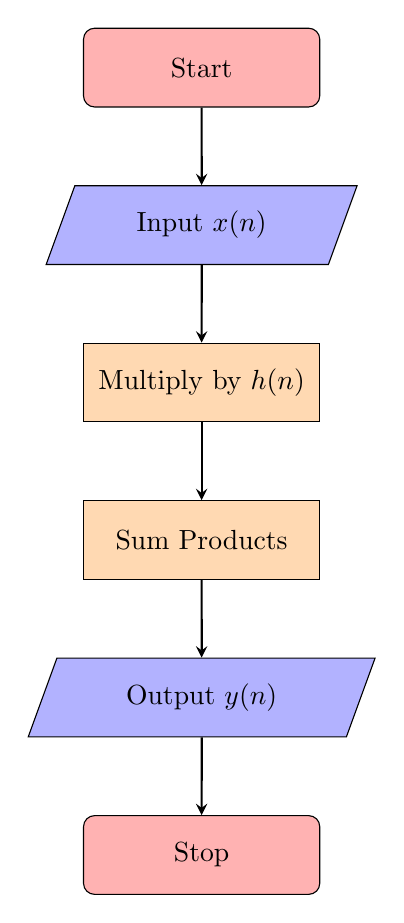
\begin{tikzpicture}[node distance=2cm]
    
    \node (start) [startstop] {Start};
    \node (in1) [io, below of=start] {Input \(x(n)\)};
    \node (pro1) [process, below of=in1] {Multiply by \(h(n)\)};
    \node (pro2) [process, below of=pro1] {Sum Products};
    \node (out1) [io, below of=pro2] {Output \(y(n)\)};
    \node (stop) [startstop, below of=out1] {Stop};
    
    \draw [arrow] (start) -- (in1);
    \draw [arrow] (in1) -- (pro1);
    \draw [arrow] (pro1) -- (pro2);
    \draw [arrow] (pro2) -- (out1);
    \draw [arrow] (out1) -- (stop);
    
    \end{tikzpicture}
    \end{center}
    
\subsection*{Part c) Find a “relatively simple” expression for the magnitude response of the filter.}

The magnitude response of an FIR filter is the absolute value of the Fourier Transform of its impulse response:
\[ H(f) = \left| \sum_{n=0}^{N-1} h(n) e^{-j2\pi fn} \right| \]

\subsection*{Part d) Write the equation for \(y(n)\) as a function of the input signal \(x(n)\) and the filter coefficients
\(h(k)\).}

The output \(y(n)\) of an FIR filter as a function of input signal \(x(n)\) and filter coefficients \(h(k)\) is:
\[ y(n) = \sum_{k=0}^{N-1} h(k) \cdot x(n-k) \]

\subsection*{Part e) The signal \(x(t) = 2\cos(2\pi125t) + \cos(2\pi250t)\) is sampled at the rate 1000samp/sec and sent into the filter. Find an expression for the steady-state output y(n) out of the filter.}

Given \(x(t) = 2\cos(2\pi125t) + \cos(2\pi250t)\) and sampling rate of 1000 samples/sec, to find \(y(n)\), we apply the filter to the discrete version of \(x(t)\), which involves convolving \(x(n)\) with \(h(n)\).

Discretizing \(x(t)\), we get:

\[x(n) = 2\cos\left(\frac{\pi}{4}n\right) + \cos\left(\frac{\pi}{2}n\right)\]

This student is assuming the filter is really good at letting signals with a lower pitch (or frequency) through without changing them much, but it blocks higher pitch sounds. Since our filter's cutoff is at 250 Hz, it will let the lower pitch part of our signal through and block the higher pitch part.

So, after filtering, the part of our signal that's like a lower frequency, \(2\cos\left(\frac{\pi}{4}n\right)\), gets through without much change, but the higher pitch sound, \(\cos\left(\frac{\pi}{2}n\right)\), might not get through at all.

simply, the output \(y(n)\) of our filter, which is what we hear or see after the filter does its job, will mostly be:

\[y(n) \approx 2\cos\left(\frac{\pi}{4}n\right)\]

This means the filter keeps the lower pitch sound pretty much the same as it was, but we don't hear the higher pitch sound after the filter.

This student assumes the filter does a perfect job of separating the lower pitch from the higher pitch sounds, which is an ideal situation. In real life, filters are not be perfect, but this gives a good idea of what to expect.

\subsection*{Part f) What is the delay (in ms) and what is the phase shift (in radians) of the two frequency
components through the filter?}

The delay and phase shift introduced by the filter can be understood in terms of group delay and the filter's phase response. For our FIR filter with length \(N = 11\), the group delay \(\tau\) is calculated as half the filter length minus one, which gives:

\[ \tau = \frac{N-1}{2} = \frac{11-1}{2} = 5 \, \text{samples} \]

To convert this delay into milliseconds (ms) at a sampling rate of 1000 samples/sec, we find:

\[ \text{Delay (ms)} = \frac{\tau}{f_s} \times 1000 = \frac{5}{1000} \times 1000 = 5 \, \text{ms} \]

The phase shift for a frequency component \(f\), in radians, is related to the group delay by:

\[ \phi = -2\pi f \tau \]

Applying this to our signal components at \(125\) Hz and \(250\) Hz:

- For \(125\) Hz, the phase shift is \(\phi_{125} = -\frac{\pi}{4} \, \text{radians}\).
- For \(250\) Hz, the phase shift is \(\phi_{250} = -\frac{\pi}{2} \, \text{radians}\).

\subsection*{Part g) Explain the impact of the use of another window function such as Hamming on the magnitude
frequency response}

Using a Hamming window instead of a rectangular window affects the filter's magnitude response, especially in terms of side lobe levels and transition width. The Hamming window reduces side lobes but increases the transition band width compared to the rectangular window.

\subsection*{Part h) The signal \(x(t) = 2\cos(2\pi100t)\) is sampled with sampling frequency 1000 Hz and sent into
the averaging FIR filter that has impulse response \(h(n) = \{-1, -1, -1, -1, -1\}\). Find the
out of the filter \(y(n)\).
}
Given the signal \(x(t) = 2\cos(2\pi100t)\) sampled with a frequency of 1000 Hz and an averaging FIR filter with impulse response \(h(n) = \{-1, -1, -1, -1, -1\}\), we aim to find the output \(y(n)\) of the filter.

\subsubsection*{Step 1: Discretization of the Input Signal}

The input signal is discretized using the sampling frequency of 1000 Hz:

\[x(n) = 2\cos\left(2\pi100 \cdot \frac{n}{1000}\right) = 2\cos\left(\frac{\pi}{5}n\right)\]

\subsubsection*{Step 2: Convolution with \(h(n)\)}

The output \(y(n)\) is determined by convolving the discretized input signal \(x(n)\) with the filter's impulse response \(h(n)\):

\[y(n) = (x * h)(n) = \sum_{k=0}^{4} x(n-k) \cdot (-1)\]

Given the specific form of \(x(n) = 2\cos\left(\frac{\pi}{5}n\right)\), this operation effectively sums up five consecutive samples of \(x(n)\), each multiplied by -1, due to the impulse response of the filter. The convolution process applies this operation across the entire length of the input signal.

The exact expression for the output \(y(n)\) is:

\[y(n) = -\sqrt{2\sqrt{5} + 10}\sin\left(\frac{\pi n}{5}\right) - \sqrt{10 - 2\sqrt{5}}\sin\left(\frac{\pi n}{5}\right) - 2\cos\left(\frac{\pi n}{5}\right)\]

This result demonstrates the filter's effect on the input signal, producing an output that is a combination of sinusoidal components with altered amplitudes and phases.

\end{document}
